\section{Multigrid Solver}
	Since the most important property of any type of solver is its correctness we have
	employed a variety of different methods to verify the multigrid solver.
	On the lowest level there is a suite of unittests that checks the modular parts
	of the algorithm where possible, see \cref{sec:unittests} for an overview.

	To test the solver itself we employ a couple different techniques. First we
	create a charge distribution by differentiating a known potential, and then
	running the solver and check if the resulting potential was equal to the original
	known potential.

	For the second test we use a charge potential with a known analytical solution,
	and we then check that the solver reproduces the known analytical solution.

	A third method we use to verify it is to produce a random charge potential
	and then check that the potential converges, or in other words
	that the residual goes toward zero.

	Then lastly we use the solver on identical charge distributions with the domain
	divided up into different subdomains and check that the solver produces the same
	potential.

\subsection{Predetermined Potential}
		In this section we first decide which potential we want, then numerically
		construct a corresponding charge potential by derivating. Then we compare the
		result with the original potential.

		In

		\begin{figure}
			\centering
			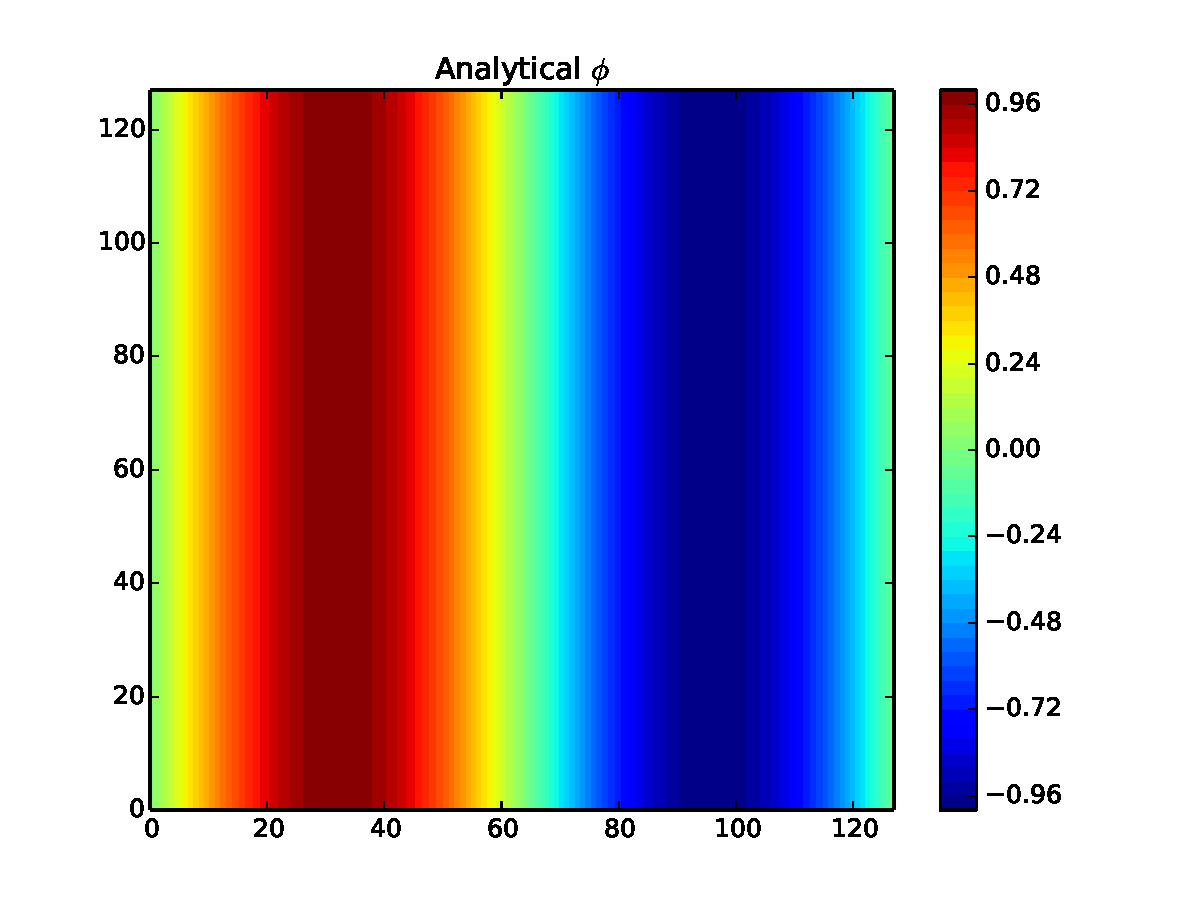
\includegraphics[width = 0.45\textwidth]{figures/verification/sinusoidal/analytical.pdf}
			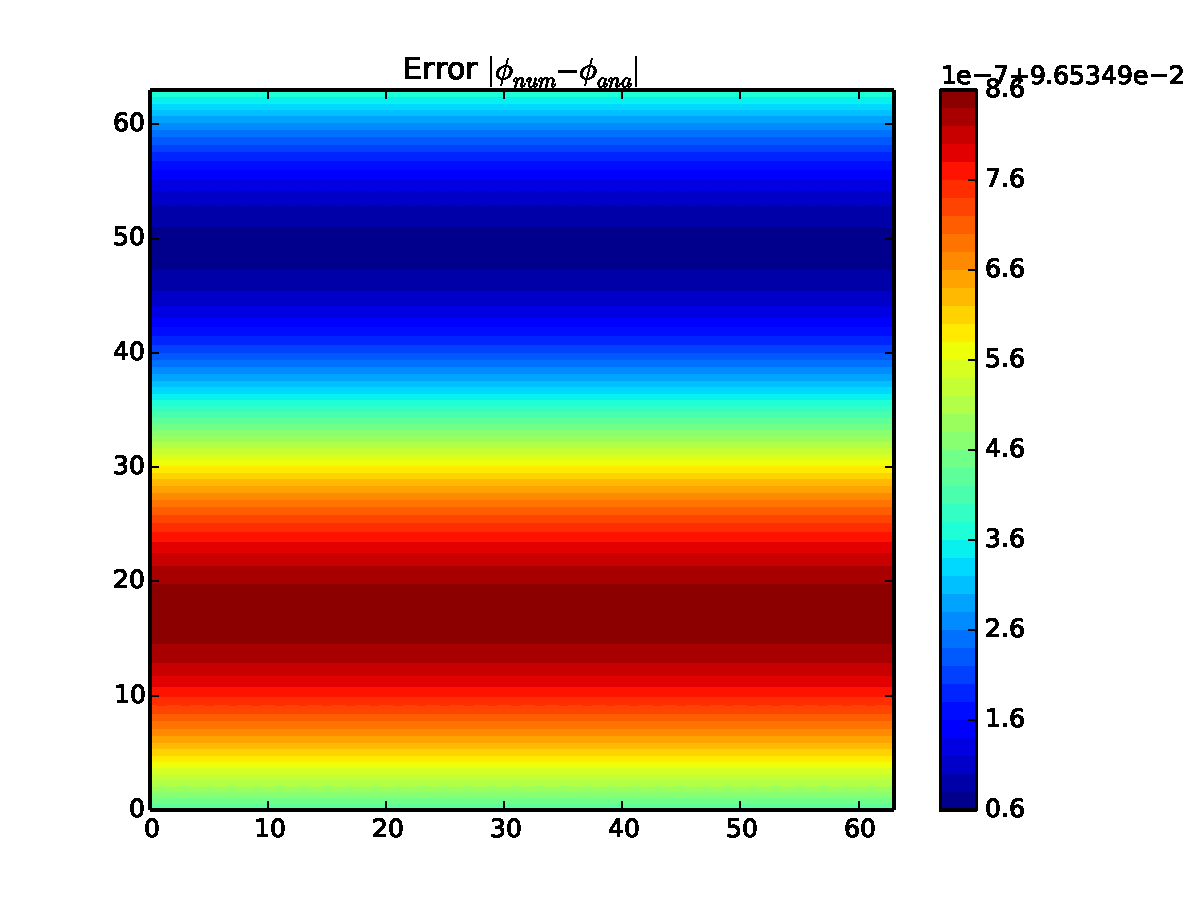
\includegraphics[width = 0.45\textwidth]{figures/verification/sinusoidal/error.pdf}
		\end{figure}


\subsection{Analytical Solutions}

		\begin{equation}
			f(x) =
		\end{equation}


\subsection{Convergence of Residual}

\subsection{Different Domain divisions}



\textbf{NB! See if something below is salvageable}


The multigrid method has several different steps in the algorithm, as a developmental
help and to ensure that the program works correctly during as many different conditions
as possible we want to test the whole code, as well as the constituent parts where possible.
The method is quite modular and several parts of it can be tested alone.
The GS-RB, used for smoothing, can be independently tested, since on it's own it converges to a solution,
just at a higher computational cost than the multigrid method. To test it we will
use an initial density field with a length between the grid steps that results in
an exact answer. The restriction and prolongation operators can also tested to a
degree by checking that they preserve a constant grid through several grid level changes.


The multigrid method has several different steps in the algorithm, as a developmental
help and to ensure that the program works correctly during as many different conditions
as possible we want to test the whole code, as well as the constituent parts where possible.
The method is quite modular and several parts of it can be tested alone.
The GS-RB, used for smoothing, can be independently tested, since on it's own it converges to a solution,
just at a higher computational cost than the multigrid method. To test it we will
use an initial density field with a length between the grid steps that results in
an exact answer. The restriction and prolongation operators can also tested to a
degree by checking that they preserve a constant grid through several grid level changes.

\subsection{The Multigrid method}
	We use both of the aforemented tests to check that the whole multigrid method
	works as intended. Since a constant source term will give a trivial solution of
	the potential, \(\phi(x,y,z) = \va{0}\), we use that as a test. In addition we
	also test that it converges on a sinusoidal source term as we did the smoother.

\subsection{Prolongation and Restriction}


	The prolongation and restriction operators with the earlier proposed stencils
 	will average out the grid points when applied. So the idea here is to set up a
 	system with a constant charge density, \(\rho(\va{r}) = C\), and then apply a
	restriction. After performing the restriction we can check that the grid points
	values are preserved. Then we can do the same with the prolongation. While this
	does not completely verify that the operators work as wanted, it gives an indication
	that we have not lost any grid points and the total mass of the charge density should be conserved.

\subsection{Smoothers}

	The iterative method GS-RB used for the pre- and postsmoothing of the grid in
	our implementation of the multigrid method is also a direct solver.
	So we can test it, or most other smoothers, by testing them on a small system
	where the problem has an analytical solution. Then we can let them run for a
	while and ensure that they are converging towards the solution. If we let
	the source term be sinusoidal in one direction, and constant in the other
	directions it has an easy solution given below

	\begin{align}
		\nabla^2 \phi(x,y,z) &= \sin(x)
	\end{align}

	This has a solution when \(\phi(x,y,z) = -\sin(x)\) and we can test that the
	solver converges to the solution. If we let the source term be constant in the
	x direction and instead vary in the other directions we can get verify that the
	solver works in all three directions independently.
